\chapter{ChessWay SL} \label{chap:chesswaysl}

\section{Case Description}
The ChessWaySL model is an extension of the previous model (see
Chapter \ref{chap:chesswaysimple}), and acts as a bridge between the
very simple model presented there and the much more complex model of
the same scooter which is presented in the following chapter (Chapter
\ref{chap:chesswaydestecs}).  The model in this chapter includes the
same basic features of a self-balancing scooter described in Chapter
\ref{chap:chesswaysimple}.  However, in this model we are beginning
the process of adding some extra safety features, additional controls
and some fault tolerant functionality. As with the previous model, the
ChessWaySL scooter consists of a platform on which the rider stands,
with two parallel wheels and a handlebar. There is an ignition switch
which the user can use to power the system down explicitly. There is
also a removable safety key device, which is always inserted into a
slot in the handlebar unit while the scooter is in use. At the same
time the safety key will be attached to the user's wrist by a cord, so
that if the user is unfortunate enough to fall off the scooter, the
safety key will be pulled away from its slot in the handlebar
unit. The removal of the safety key can therefore assumed to mean that
the scooter is riderless, and the vehicle must immediately come to a
safe, stationary position.

A distributed controller architecture was chosen for the more advanced
ChessWay, whereby each wheel has its own controller. Each motor
controller is guarded by a so-called safety monitor, which has the
task to intervene and put the system in a fail-safe state in case any
fault is detected. The failsafe state condition for the ChessWay is
the situation where neither motor is actuated. Furthermore, the system
should be able to recuperate from such an intervention and return to
normal operating mode, in case the root cause of the fault has been
removed.  Figure \ref{fig:controllerstates} shows the states and
transitions we require for the controller, and Figure
\ref{fig:plantstates} shows the events and transitions needed for the
plant.
\begin{figure}[!ht ]
\centering
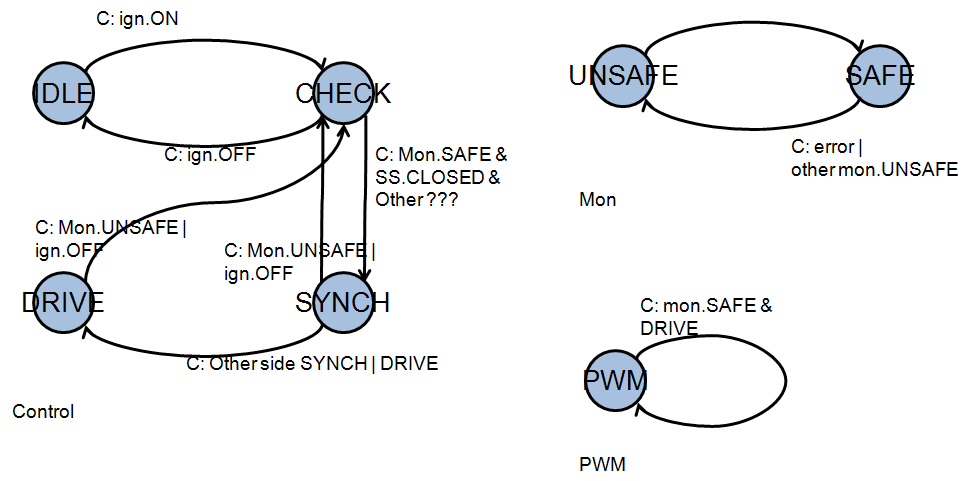
\includegraphics[width=1\textwidth]{chessWaySL/StatesForController.png}
\caption{States and transistions needed for the ChessWay controller model
\label{fig:controllerstates}}
\end{figure}

\begin{figure}[!ht ]
\centering
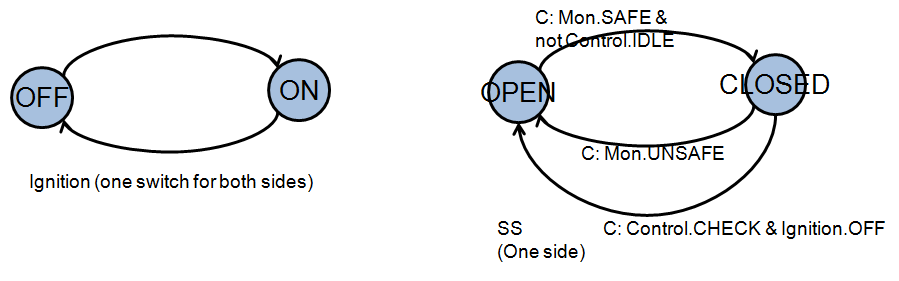
\includegraphics[width=1\textwidth]{chessWaySL/StatesForPlant.png}
\caption{States and transistions needed for the ChessWay plant model
\label{fig:plantstates}}
\end{figure}

In order to develop the simple version of the model (Chapter
\ref{chap:chesswaysimple}) into a model that incorporates all of the
above features, some key design questions must be answered:

\begin{itemize}
\item What constitutes the system?
\item What constitutes the environment?
\item What should constitute the DE side of the simulator?
\item What should constitute software in the controller?
\item What is the minimum number of sensors we need and what is
  necessary for the plant?
\end{itemize}

In order to answer these questions, engineers initially adopt a
DE-first approach, designing the DE side of the model only and
assuming that there is a CT model available which is always correct.
This allows them to concentrate on the discrete event changes that
will be encountered during start-up and shut down, and during
fault-handling and recovery.  The added value of the intermediate
model is that is focuses on state changes only: it shows which sensors
are deeded to be able to detect certain faults; it changes state from
detecting a fault to a safe sate and tries to recover to an
operational state; and it shows the interaction between user and
device.  We present the intermediate, DE-only model in this chapter,
and we present a more complete version of the model with a
fully-implemented CT model in Chapter \ref{chap:chesswaydestecs}.
\section{Defining Data Types}
The first step is to define a set of data types which will act as a
convenient vocabulary in our model.  Simple types (omitted here) for
describing properties from the physical domain start with a capital
\textbf{R} and for the sensed properties we use a prefix
\textbf{S}. The actuator types are preceded by \textbf{A}.  The safety
monitor observes the system health and manages variables of type
\texttt{SafetyMode}.  The controller operates the system and manages
variables of type \texttt{OperatingMode}.

\begin{vdm_al}
	types
		Plant ::
			poleAngle : RPoleAngle
			angleVel : RAngleVel
			safetyKey : RSafetyKey
			powerSwitch : RPowerSwitch
			pwmL : RPwm
			pwmR : RPwm
			safetySwitchL : RSafetySwitch
			safetySwitchR : RSafetySwitch;

		Sensors ::
			ignition : SPowerSwitch
			poleAngle : SPoleAngle
			angleVel : SAngleVel
			safetyKey : SSafetyKey;

		Actuators ::
			pwm : APwm
			safetySwitch : ASafetySwitch;

		Controller ::
			mode : OperatingMode;

		Monitor ::
			mode : SafetyMode;
\end{vdm_al}

The structured types show that the \texttt{Plant} type holds the
actual physical properties, while \texttt{Sensors} contains the
observed values. The real and observed values may differ due to
timing, as the real physical property changes in real-time while the
sensed values only changes when triggered to do so. And furthermore,
the values may differ due to sensor faults. A similar argument holds
for the actuators.

\section{Defining State}
We can now define the state of our model (some states are omitted
here).

\begin{vdm_al}
state Sigma of
	-- real world
	plant  : Plant

	-- modelled world
	sens  : Sensors
	actL  : Actuators
	actR  : Actuators
	ctrlL : Controller
	ctrlR : Controller
	monL  : Monitor
	monR  : Monitor

	-- keep track of the error state
	errors : map ErrorTypes to bool
\end{vdm_al}

Note that the variable \texttt{plant} represents the physical system
properties.  The \texttt{sens} variable is used to hold the sampled
sensor value at some specific point in time, while the variables
\texttt{actL} and \texttt{actR} hold the most recent control signal
which is send to the motors that drive a wheel each.  Finally there is
a pair of \textit{controllers} and a pair of \textit{monitors}.  The
controller resembles the digital controller and the monitor represents
the safety monitor for that controller. The \texttt{plant} and
\texttt{sens} variables occur once, while all other system elements
occur twice, for the left (\textbf{L}) and the right (\textbf{R})
wheel respectively. The controller and monitor variables are
containers for the controller and monitor state machines. They will
become the core processes in co-simulation and in the implementation.

\section{Defining Auxiliary Functions}
We can now define some auxiliary functions and operations that can be
used as encodings of transitions in a state machine.  Using some
simple functions (omitted here) to read sensors, whereby we treat the
user interface button (on/off switch) as an ordinary sensor, we can
now define the transition engine that is at the heart of the
controller state machine.

\begin{vdm_al}
  -- process to migrate from state to state = statemachine
  switchState : Controller * Monitor * Actuators *
    Controller * Monitor ==> OperatingMode
  switchState(c, m, act, cOther, mOther) == (
      -- check monitor first
      -- check ignition
      -- change state
      cases c.mode :
        <IDLE> ->  if sens.ignition = <OFF>
                   then return <IDLE>
                   else return <CHECK>,
        <CHECK> -> if sens.ignition = <OFF>
                   then return <IDLE>
                   else if m.mode = <SAFE> and
                           act.safetySwitch = <CLOSED>
                        then return <SYNC>
                        else return <CHECK>,
        <SYNC> -> ( if m.mode = <SAFE> and
                       mOther.mode = <SAFE> and
                       ( cOther.mode = <SYNC> or
                         cOther.mode = <DRIVE> )
                    then return <DRIVE>;
                    if m.mode <> <SAFE> or
                       mOther.mode <> <SAFE>
                    then return <CHECK>;
                    return <SYNC> ),
        <DRIVE> -> if m.mode <> <SAFE> or
                      sens.ignition = <OFF>
                   then return <CHECK>
                   else return <DRIVE>
      end;
      -- default return value
      return <CHECK>;
    );
\end{vdm_al}

The core process of the controller. The On/Off switch makes the state
switch between \textsf{IDLE} and the other states.  The \textsf{CHECK}
state is the landing place after switching on and after detection of
an error. The \textsf{SYNC} state is introduced to synchronize between
the left and right controller. The controller being in a safe state, a
check is made before powering the motor that the other side is in the
same state as well. If so then both will move to the \textsf{DRIVE}
state and power the two motors. In case of an error, or desire to
switch off, the mode will change to \textsf{CHECK} again.

\section{Usage}
Finally,
we can create an operation that simulates the behavior of the state
machine.
\begin{vdm_al}
  -- simulator
  simulator : () ==> ()
  simulator() == (
    dcl tick : int := 0;

    while tick < 25 do (
      IO`print(tick);

      -- script
      if tick = 2
        then switchOn();
      if tick = 4
        then pullSafetyKey();
      if tick = 7
        then restoreSafetyKey();
      if tick = 16
        then pullSafetyKey();
      if tick = 19
        then restoreSafetyKey();
      if tick = 23
        then switchOff();

      -- read sensor values
      sens := sense();

      -- sense & monitor & activate
      if ctrlL.mode <> <IDLE>
        then (
          monL.mode := switchMonitorState(ctrlL);
          actL.safetySwitch :=
            switchSafetySwitch(monL.mode, ctrlL.mode);
          actL.pwm := pwmOut(ctrlL.mode, monL.mode, sens);
          plant.pwmL := setPwm(actL);
          plant.safetySwitchL := setSafetySwitch(actL);
      );
      if ctrlR.mode <> <IDLE>
	    then (
          monR.mode := switchMonitorState(ctrlR);
          actR.safetySwitch :=
            switchSafetySwitch(monR.mode, ctrlR.mode);
          actR.pwm := pwmOut(ctrlR.mode, monR.mode, sens);
          plant.pwmR := setPwm(actR);
          plant.safetySwitchR := setSafetySwitch(actR)
        );

      -- control
      ctrlL.mode := switchState(ctrlL, monL, actL, ctrlR, monR);
      ctrlR.mode := switchState(ctrlR, monR, actR, ctrlL, monL);

      tick := tick + 1;
    );
  )
end Chessway
\end{vdm_al}

The simulator process demonstrates that changes in the environment
(user input) make the system pass the states in a desired
manner. Switch \textsf{On} and \textsf{Off}, and pulling the safety
key at specific moments to trigger errors at all times in the state
machine.  Code coverage analysis showed that initial tests missed some
of the possible execution paths. By adding more tests manually, more
confidence is gained in the design and analysis. The experiments show
that this model is at the right level of being able to add faults and
to analyse fault handling.

